In the discussion of the paper by \citet{GilmourTrinca2012}, among many comments and suggestions, two of them are of our particular interest if we research the ways of constructing optimality criteria reflecting various desirable inference properties:
\begin{itemize}
\item Designs which were obtained by optimising according to the $DP$- and/or $LP$-criterion tend to have most of the residual degrees of freedom allocated to the pure error component in the error variance decomposition thus creating an imbalance and even making the test for lack of fit impossible in the extreme case, when all available degrees of freedom are assigned to pure error. In Section \ref{sec::extraF} we consider an amendment of the criteria that could potentially result in some improvements.
\item In the construction of a compound criterion each component is essentially the identity function of an elementary efficiency; in other words, the impact of each individual component is proportional to the corresponding efficiency value. However, in some situations it might be sensible to alter the nature of this impact, for example, `cut off' the designs that perform below a certain threshold with respect to a particular component or, on the contrary, assume that all designs with efficiencies large enough are equally `good'. In Section \ref{sec::desfun} we will employ some desirability functions as the compound criterion components and will examine how this would affect the results. 
\end{itemize} 

\section{Extra F-quantile}
\label{sec::extraF}
If we are in the framework of an unblocked experiment and the fitted model is polynomial regression with $p$ parameters (\ref{eq::back_model}):
\begin{equation*}
\bm{Y}=\bm{\beta}_{0}+\bm{X\beta}+\bm{\varepsilon},
\end{equation*}
i.e. $p-1$ parameters of interest and the intercept being the nuisance parameter, we can decompose the full information matrix:
\begin{equation*}
%\label{eq::infmatrix}
\bm{M}=\left[ \begin{array}{c}\bm{1'}\\\bm{X'}\end{array} \right]\left[\begin{array}{cc}\bm{1} & \bm{X}\end{array}\right]=\left[\begin{array}{cc}
\bm{n} & \bm{1'X}\\ \bm{X'1} & \bm{X'X} 
\end{array}  \right].
\end{equation*}
Then the information matrix corresponding to all parameters except for the intercept, will look as follows:
\begin{equation}
\label{eq::s_infmatrix}
(\bm{M}^{-1}_{22})^{-1}=\bm{X'}\bm{Q}_{0}\bm{X}, \mbox{ where }\bm{Q}_{0}=\bm{I_n}-\frac{1}{n}\bm{11'}.  
\end{equation}
This representation is essentially a special case of the blocked experiment framework, described in Section \ref{sec::back_blocked}, with matrix of block indicators $\bm{Z}$ being an $(n\times 1)$ intercept column. 

Therefore the corresponding `pure error' optimality criteria  become (see also (\ref{eq::DPs_blocked}) and (\ref{eq::LPs_blocked})): 
\begin{align}
\label{eq::DPs_inter}
DP_S: \mbox{minimise } &(F_{p-1,d;1-\alpha_{DP}})^{p-1}\vert (\bm{X'}\bm{Q}_{0}\bm{X})^{-1}\vert,\\
\label{eq::LPs_inter}
LP_S: \mbox{minimise } &F_{1,d;1-\alpha_{LP}}\mbox{tr}\{\bm{W}(\bm{X'}\bm{Q}_{0}\bm{X})^{-1}\}.
\end{align}

Martina Vandebroek in the discussion of the paper by \cite{GilmourTrinca2012} (p.~$373$) suggested including an extra $F$-quantile as a compound criterion component which would guarantee some degrees of freedom for both pure error and lack-of-fit parts. 

To test the model for the lack of fit, the following test statistic might be used:
\begin{equation*}
\frac{LoF\mbox{ }SS/(n-p-d)}{Pure\mbox{ }Error\mbox{ }SS/d} \sim F_{n-p-d,d}.
\end{equation*}
In a similar way as before, the `lack-of-fit', $LoF$-efficiency can be defined:
\begin{equation}
\label{eq::LoF_eff}
\mbox{Eff}_{LoF}(\bm{X})=\frac{F_{n-p-d_{*},d_{*};1-\alpha_{LoF}}}{F_{n-p-d,d;1-\alpha_{LoF}}},
\end{equation}
where $d_{*}$ is the number of pure error degrees of freedom of the optimal design $\bm{X}_{*}$ in terms of maximising $1/F_{n-p-d,d;1-\alpha_{LoF}}$ or, equivalently, minimising $F_{n-p-d,d;1-\alpha_{LoF}}$. The scale of such representation is in accordance with the previously defined $D$-efficiency in (\ref{eq::D_eff}), and with the accordingly defined $DP_S$-efficiency:
\begin{equation}
\mbox{Eff}_{DP_S}(\bm{X})=\frac{F_{p-1,d_{*};1-\alpha_{DP}}\vert(\bm{X_{*}}'\bm{Q}_{0}\bm{X_{*}})^{-1}\vert ^{1/p-1}}{F_{p-1,d;1-\alpha_{DP}}\vert(\bm{X}'\bm{Q}_{0}\bm{X})^{-1}\vert ^{1/p-1}}.
\end{equation}

In Figure \ref{Fig::extraF} the values of the inverse $F$-quantile are presented depending on the pure error degrees of freedom for three different scenarios of available residual degrees of freedom: $19$, $25$ and $30$. In all cases the curvatures are clearly convex, so that maximum values exist and they are unique in every given case. Larger numbers of available residual degrees of freedom correspond to the larger `optimal' pure error degrees of freedom, i.e. where the maximum of the inverse F-quantile is achieved. For example, when $n-p$ is equal to $19$, the optimal $d$ is $12$, and for $n-p=30$ the maximum of $F_{n-p-d,d;1-\alpha_{LoF}}$ is at $d=19$.

% F-percentile
\begin{figure}[ht]
\begin{center}
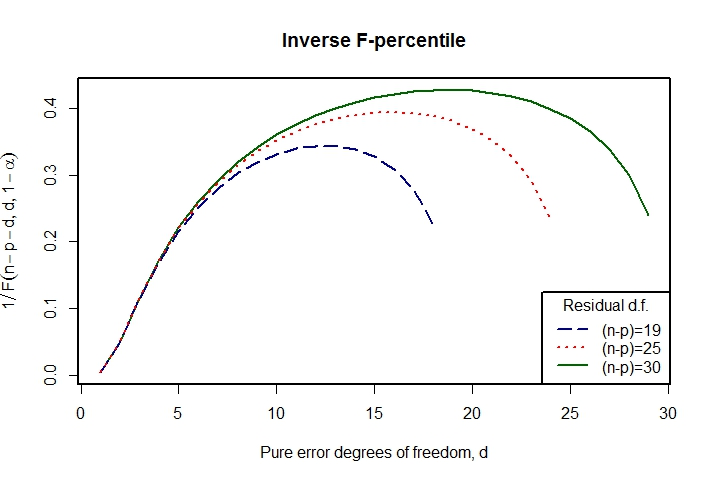
\includegraphics[scale=0.7]{Fquantile.jpeg}
\caption{Inverse F-quantile vs Pure Error degrees of freedom, $d$}
\label{Fig::extraF}
\end{center}
\end{figure}

Adding this element (\ref{eq::LoF_eff}) to the components responsible for the point and interval precision of the parameters' estimates: $D_S$ and $DP_S$ (or $L_S$ and $LP_S$) and the $DF$ criterion defined in (\ref{eq::DF_eff}), we get the following determinant and trace-based functions to be minimised:
\begin{align}
\label{eq::ExtraFD_crit}
\vert\bm{X}'\bm{Q_{0}}\bm{X}\vert^{-\frac{\kappa_D}{(p-1)}}\times \left[F_{p-1,d;1-\alpha_{DP}}\vert\bm{X'}\bm{Q_{0}}\bm{X}\vert^{-\frac{1}{(p-1)}}\right]^{\kappa_{DP}}\times(n-d)^{\kappa_{DF}}\times \notag \\ \left[F_{n-p-d,d;1-\alpha_{LoF}}\right]^{\kappa_{LoF}}
\end{align}
and
\begin{align}
\label{eq::ExtraFL_crit}
\left[\mbox{trace}\{\bm{W}(\bm{X'}\bm{Q_{0}}\bm{X})^{-1}\}\right]^{\kappa_L+\kappa_{LP}}\times\left[F_{1,d;1-\alpha_{LP}}\right]^{\kappa_{LP}}\times (n-d)^{\kappa_{DF}}\times\left[F_{n-p-d,d;1-\alpha_{LoF}}\right],^{\kappa_{LoF}}
\end{align}
where, as before, $d$ stands for the number of pure error degrees of freedom or, equivalently, the number of replicated points in the model matrix $\bm{X}$. The significance levels $\alpha_{DP}$ and $\alpha_{LoF}$ are usually set to $0.05$; correction for multiple comparisons is applied to the $LP_s$-component, as given in (\ref{eq::Sidak}), and $\alpha_{LP}$ is amended accordingly. The third component in both criteria corresponds to the DF-efficiency defined in (\ref{eq::DF_eff}).
 
\subsection{Optimal designs accounting for the model lack-of-fit}
\label{sec::optimal_extraF}
The following example was considered in order to compare optimal designs obtained for various compound criteria consisting of weighted combinations of $D_S$-, $DP_S$-, $DF$- and $LoF$-efficiencies. 
Designs were derived for a factorial experiment with five explanatory factors, each of three levels, and with only $40$ runs. The full second-order polynomial model is to be fitted, i.e. the number of parameters $p=21.$ The intercept is a nuisance parameter, and so further on we will be dealing with optimality criteria only for the parameters of interest. However, in the notation the subscript $S$ shall be omitted.

The resulting design is to be chosen (in other words, sampled with replacement) from the candidate set of points containing $3^{5}=243$ possible combinations of factors' values. A standard point exchange algorithm with $500$ random starts was used to find the optimal combination (as described before and the same as was used in \citealp{GilmourTrinca2012}).

In Table \ref{Table_extraFD} each row corresponds to the optimal design obtained with respect to the criterion function (\ref{eq::ExtraFD_crit}) with the weights given in the first columns; then the degrees of freedom (DoF) for pure error (PE) and lack of fit (LoF) are presented together with the individual efficiencies of the designs. Zero values there indicate the cases when a certain component ($DP$, $LP$ or $LoF$) cannot be estimated due to the absence of replicates in the design. 

Some expected features might be noticed here: designs which perform well in terms of the $D$-criterion generally have quite large $L$-efficiency values (and a similar tendency holds for $DP$- and $LP$-efficiencies). When all the components are equally weighted (design \#$12$), the resulting design performs well in terms of all the criteria, all efficiencies are above $90\%$.  

\begin{table}[h]
\centering
\caption{Example 1. Properties of optimal designs with respect to determinant-based compound criteria with an extra F-quantile}
\label{Table_extraFD}
\scalebox{0.8}{
%\resizebox{\textwidth}{!}} \\
\multicolumn{1}{l}{} & \textbf{D} & \textbf{DP} & \textbf{DF} & \textbf{LoF} & \textbf{PE} & \textbf{LoF} & \textbf{D} & \textbf{DP} & \textbf{L} & \textbf{LP} & \textbf{LoF} & \textbf{DF}\\
1 & 1 & 0 & 0 & 0 & 0 & 19 & 100.00 & 0.00 & 99.67 & 0.00 & 0.00 & 100.00 \\
2 & 0 & 1 & 0 & 0 & 18 & 1 & 93.00 & 100.00 & 79.32 & 93.01 & 66.00 & 55.00\\
3 & 0.5 & 0.5 & 0 & 0 & 16 & 3 & 95.29 & 98.64 & 79.96 & 92.09 & 89.95 & 60.00 \\
4 & 0.5 & 0 & 0.5 & 0 & 0 & 19 & 100.00 & 0.00 & 99.67 & 0.00 & 0.00 & 100.00\\
5 & 0.5 & 0 & 0 & 0.5 & 12 & 7 & 97.59 & 90.38 & 90.24 & 98.39 & 100.00 & 70.00\\
6 & 0 & 0.5 & 0.5 & 0 & 12 & 7 & 97.62 & 90.40 & 90.63 & 98.81 & 100.00& 70.00\\
7 & 0 & 0.5 & 0 & 0.5 & 14 & 5 & 96.93 & 95.61 & 88.12 & 98.19 & 98.48 & 65.00\\
8 & 0 & 0 & 0.5 & 0.5 & 10 & 9 & 49.77 & 42.27 & 25.19 & 26.26 & 96.46 & 75.00\\
9 & 1/3 & 1/3 & 1/3 & 0 & 12 & 7 & 97.60 & 90.38 & 90.19 & 98.33 & 100.00& 70.00\\
10 & 1/3 & 1/3 & 0 & 1/3 & 14 & 5 & 96.93 & 95.61 & 87.27 & 98.19 & 98.48 & 65.00\\
11 & 0 & 1/3 & 1/3 & 1/3 & 12 & 7 & 97.60 & 90.38 & 90.19 & 98.33 & 100.00 & 70.00\\
12 & 0.25 & 0.25 & 0.25 & 0.25 & 12 & 7 & 97.62 & 90.40 & 90.63 & 98.81 & 100.00 & 70.00\\
\end{tabular}
}
\end{table} 
It is also noticeable that the $D$-optimal design (\#$1$) retains its optimality when half of the weight is allocated to the $DF$-component, i.e. with $\kappa_{D}=\kappa_{DF}=0.5$ (\#$4$), and it contains no replicates. The design itself is presented in Table \ref{tab::design1} (with the points ordered for the sake of perception): it can be seen that the design points are more or less evenly distributed over the design space, with one centre point and with half of the points being `corner' ones, i.e. when all factors take the values $\pm1$. 

All other designs have more degrees of freedom allocated to the pure error component than to the lack-of-fit one and, therefore, their $DF$-efficiency values $\frac{n-d}{n}$ are below $75\%$ (i.e. when $d>10$). The maximum of the lack-of-fit efficiency is achieved when $d=12$, and the balance in the allocation of degrees of freedom was obtained when the total weight was equally distributed between the $DF$- and $LoF$-components, so that design \#$8$ given in the table is quite arbitrary and can be replaced with any other having $10$ pure error degrees of freedom. Further improvements of the performance in terms of other components can be achieved, for example, by setting a constraint on the degrees of freedom.
\begin{table}[h]
\centering
\caption{Example 1. D-optimal design (\#$1$ and \#$4$)}
\label{tab::design1}
\scalebox{0.8}{
\begin{tabular}{rrrrrr|r|rrrrrr}
1  & -1 & -1 & -1 & -1 & 1  &  & 21 & 0 & 1  & -1 & -1 & -1 \\
2  & -1 & -1 & -1 & 1  & -1 &  & 22 & 0 & 1  & 0  & -1 & 1  \\
3  & -1 & -1 & -1 & 1  & 1  &  & 23 & 0 & 1  & 1  & 1  & -1 \\
4  & -1 & -1 & 0  & -1 & -1 &  & 24 & 1 & -1 & -1 & -1 & -1 \\
5  & -1 & -1 & 1  & -1 & 1  &  & 25 & 1 & -1 & -1 & -1 & 1  \\
6  & -1 & -1 & 1  & 1  & -1 &  & 26 & 1 & -1 & -1 & 1  & 0  \\
7  & -1 & -1 & 1  & 1  & 1  &  & 27 & 1 & -1 & 0  & 0  & 1  \\
8  & -1 & 0  & -1 & -1 & -1 &  & 28 & 1 & -1 & 1  & -1 & -1 \\
9  & -1 & 0  & 1  & 0  & -1 &  & 29 & 1 & -1 & 1  & 1  & -1 \\
10 & -1 & 1  & -1 & -1 & 0  &  & 30 & 1 & -1 & 1  & 1  & 1  \\
11 & -1 & 1  & -1 & 0  & 1  &  & 31 & 1 & 0  & -1 & -1 & 0  \\
12 & -1 & 1  & -1 & 1  & -1 &  & 32 & 1 & 0  & 0  & 1  & -1 \\
13 & -1 & 1  & 0  & 1  & 0  &  & 33 & 1 & 0  & 1  & -1 & 1  \\
14 & -1 & 1  & 1  & -1 & -1 &  & 34 & 1 & 1  & -1 & -1 & 1  \\
15 & -1 & 1  & 1  & -1 & 1  &  & 35 & 1 & 1  & -1 & 0  & -1 \\
16 & -1 & 1  & 1  & 1  & 1  &  & 36 & 1 & 1  & -1 & 1  & -1 \\
17 & 0  & -1 & -1 & 0  & -1 &  & 37 & 1 & 1  & -1 & 1  & 1  \\
18 & 0  & -1 & 1  & -1 & 0  &  & 38 & 1 & 1  & 1  & -1 & -1 \\
19 & 0  & 0  & -1 & 1  & 1  &  & 39 & 1 & 1  & 1  & 0  & 0  \\
20 & 0  & 0  & 0  & 0  & 0  &  & 40 & 1 & 1  & 1  & 1  & 1 
\end{tabular}
}
\end{table} 
Whether equal weights are distributed between $DP$ and $LoF$ components of the compound criterion or between $D$, $DP$ and $LoF$, the resulting designs are the same (\#$7$ and \#$10$), providing quite large $DP$-, $LP$- and $LoF$-efficiency values and fairly high $D$-efficiency. The design can be found in Table \ref{tab::design7}: all of its pure error degrees of freedom occur from the single replicates of the corner points, there is no centre point and in general fewer points contain any factors at the zero level in comparison to the $D$-optimal design observed before.

\begin{table}[h]
\centering
\caption{Example 1. Optimal design with respect to the determinant based-criteria \#$7$ and \#$10$}
\label{tab::design7}
\scalebox{0.8}{
\begin{tabular}{rrrrrr|r|rrrrrr}
1  & -1 & -1 & -1 & -1 & 1  &  & 21 & 0 & 0  & -1 & -1 & 0  \\
2  & -1 & -1 & -1 & -1 & 1  &  & 22 & 0 & 0  & 0  & 1  & 1  \\
3  & -1 & -1 & -1 & 1  & -1 &  & 23 & 0 & 1  & 1  & 0  & 1  \\
4  & -1 & -1 & -1 & 1  & -1 &  & 24 & 1 & -1 & -1 & -1 & -1 \\
5  & -1 & -1 & 1  & -1 & -1 &  & 25 & 1 & -1 & -1 & -1 & -1 \\
6  & -1 & -1 & 1  & 1  & 1  &  & 26 & 1 & -1 & -1 & 1  & 1  \\
7  & -1 & -1 & 1  & 1  & 1  &  & 27 & 1 & -1 & -1 & 1  & 1  \\
8  & -1 & 0  & -1 & 0  & 0  &  & 28 & 1 & -1 & 1  & -1 & 1  \\
9  & -1 & 0  & 0  & 0  & -1 &  & 29 & 1 & -1 & 1  & -1 & 1  \\
10 & -1 & 0  & 1  & -1 & 1  &  & 30 & 1 & -1 & 1  & 1  & -1 \\
11 & -1 & 1  & -1 & -1 & -1 &  & 31 & 1 & -1 & 1  & 1  & -1 \\
12 & -1 & 1  & -1 & -1 & -1 &  & 32 & 1 & 1  & -1 & -1 & 1  \\
13 & -1 & 1  & -1 & 1  & 1  &  & 33 & 1 & 1  & -1 & -1 & 1  \\
14 & -1 & 1  & -1 & 1  & 1  &  & 34 & 1 & 1  & -1 & 1  & -1 \\
15 & -1 & 1  & 0  & -1 & 1  &  & 35 & 1 & 1  & -1 & 1  & -1 \\
16 & -1 & 1  & 1  & -1 & 0  &  & 36 & 1 & 1  & 0  & 0  & 0  \\
17 & -1 & 1  & 1  & 1  & -1 &  & 37 & 1 & 1  & 1  & -1 & -1 \\
18 & -1 & 1  & 1  & 1  & -1 &  & 38 & 1 & 1  & 1  & -1 & -1 \\
19 & 0  & -1 & 0  & -1 & 0  &  & 39 & 1 & 1  & 1  & 1  & 1  \\
20 & 0  & -1 & 1  & 0  & -1 &  & 40 & 1 & 1  & 1  & 1  & 1 
\end{tabular}
}
\end{table}
Also the same design is optimal according to the criteria \#$9$ and \#$11$ (and it is quite similar to the optimal design with respect to the equal-weighted criterion \#$12$), such that a little weight reallocation in this case does not substantially affect the performance.

Optimal designs with respect to similar trace-based criteria are presented in Table \ref{Table_extraFL}. On the whole, the relationships between the weights of the criteria and resulting designs' efficiencies are similar to the ones seen above. However, here one can observe more variability in the distribution of the degrees of freedom between the pure error and lack-of-fit components: designs \#$6$ and \#$9$ have $8$ pure error degrees of freedom, although, their $DP$-efficiencies are lower than  usual (approximately $72\%$ instead of up to $90\%$). In addition, the design optimal according to the equal-weighted criterion (\#$12$) is also optimal with respect to the criterion with equal weights put on the $DF$- and $LoF$-components as it has the balanced allocation of degrees of freedom; it is presented in Table \ref{tab::Ldesign9} below as an illustration of a compromise between the different components of the trace-based criterion.     

\begin{table}[h]
\centering
\caption{Example 1. Properties of optimal designs with respect to trace-based compound criteria with an extra F-quantile}
\label{Table_extraFL}
\scalebox{0.8}{
%\resizebox{\textwidth}{!}} \\
\textbf{} & \textbf{L} & \textbf{LP} & \textbf{DF} & \textbf{LoF} & \textbf{PE} & \textbf{LoF} & \textbf{D} & \textbf{DP} & \textbf{L} & \textbf{LP} & \textbf{LoF} & \textbf{DF} \\
1 & 1 & 0 & 0 & 0 & 0 & 19 & 99.95 & 0.00 & 100.00 & 0.00 & 0.00 & 100.00\\
2 & 0 & 1 & 0 & 0 & 14 & 5 & 95.01 & 93.72 & 88.88 & 100.00 & 98.48 & 65.00 \\
3 & 0.5 & 0.5 & 0 & 0 & 11 & 8 & 97.18 & 86.50 & 92.83 & 99.18 & 98.83 & 72.50 \\
4 & 0.5 & 0 & 0.5 & 0 & 0 & 19 & 99.95 & 0.00 & 100.00 & 0.00 & 0.00 & 100.00\\
5 & 0.5 & 0 & 0 & 0.5 & 12 & 7 & 96.69 & 89.54 & 91.71 & 99.99 & 100.00 & 70.00\\
6 & 0 & 0.5 & 0.5 & 0 & 8 & 11 & 97.10 & 72.60 & 95.61 & 93.06 & 87.94 & 80.00 \\
7 & 0 & 0.5 & 0 & 0.5 & 13 & 6 & 95.55 & 91.54 & 90.11 & 99.93 & 99.93 & 67.50 \\
8 & 0 & 0 & 0.5 & 0.5 & 10 & 9 & 49.77 & 42.27 & 25.19 & 26.26 & 96.46 & 75.00\\
9 & 1/3 & 1/3 & 1/3 & 0 & 8 & 11 & 96.75 & 72.34 & 95.35 & 92.80 & 87.94 & 80.00\\
10 & 1/3 & 1/3 & 0 & 1/3 & 12 & 7 & 96.69 & 89.54 & 91.71 & 99.99 & 100.00 & 70.00\\
11 & 0 & 1/3 & 1/3 & 1/3 & 11 & 8 & 96.65 & 86.02 & 92.74 & 99.09 & 98.83 & 72.50\\
12 & 0.25 & 0.25 & 0.25 & 0.25 & 10 & 9 & 96.91 & 82.29 & 93.99 & 97.98 & 96.46 & 75.00
\end{tabular}
}
\end{table} 

\begin{table}[h]
\centering
\caption{Example 1. Optimal design with respect to the trace based-criterion \#$12$}
\label{tab::Ldesign9}
\scalebox{0.8}{
\begin{tabular}{rrrrrr|r|rrrrrr}
1  & -1 & -1 & -1 & -1 & -1 &  & 21 & 0 & 0  & 1  & 1  & 0  \\
2  & -1 & -1 & -1 & -1 & 0  &  & 22 & 0 & 1  & -1 & -1 & -1 \\
3  & -1 & -1 & -1 & 1  & 1  &  & 23 & 0 & 1  & -1 & 1  & 0  \\
4  & -1 & -1 & -1 & 1  & 1  &  & 24 & 0 & 1  & 1  & -1 & 1  \\
5  & -1 & -1 & 1  & -1 & 1  &  & 25 & 1 & -1 & -1 & -1 & 1  \\
6  & -1 & -1 & 1  & 1  & -1 &  & 26 & 1 & -1 & -1 & -1 & 1  \\
7  & -1 & -1 & 1  & 1  & -1 &  & 27 & 1 & -1 & -1 & 1  & -1 \\
8  & -1 & 0  & -1 & 1  & -1 &  & 28 & 1 & -1 & -1 & 1  & -1 \\
9  & -1 & 0  & 0  & -1 & 1  &  & 29 & 1 & -1 & 1  & -1 & -1 \\
10 & -1 & 0  & 1  & 0  & 0  &  & 30 & 1 & -1 & 1  & -1 & -1 \\
11 & -1 & 1  & -1 & -1 & 1  &  & 31 & 1 & -1 & 1  & 1  & 1  \\
12 & -1 & 1  & -1 & 0  & 0  &  & 32 & 1 & 0  & -1 & -1 & -1 \\
13 & -1 & 1  & 0  & 1  & -1 &  & 33 & 1 & 0  & 0  & 1  & 1  \\
14 & -1 & 1  & 1  & -1 & -1 &  & 34 & 1 & 1  & -1 & 0  & -1 \\
15 & -1 & 1  & 1  & -1 & -1 &  & 35 & 1 & 1  & -1 & 1  & 1  \\
16 & -1 & 1  & 1  & 1  & 1  &  & 36 & 1 & 1  & 0  & -1 & 0  \\
17 & -1 & 1  & 1  & 1  & 1  &  & 37 & 1 & 1  & 0  & -1 & 0  \\
18 & 0  & -1 & 0  & 0  & -1 &  & 38 & 1 & 1  & 1  & 0  & 1  \\
19 & 0  & -1 & 0  & 0  & -1 &  & 39 & 1 & 1  & 1  & 1  & -1 \\
20 & 0  & 0  & -1 & 0  & 1  &  & 40 & 1 & 1  & 1  & 1  & -1
\end{tabular}
}
\end{table}

Again all the replicated points are the `corner' ones, except for the point number $18-19$ and the point number $36-37$; points are scattered across the design region, but at fewer than half of the runs at least one factor is applied at its $0$ level.

We also considered a slightly larger example of an experimental framework: four five-level factors (i.e. $625$ candidate points), $60$ runs and the full quadratic polynomial ($p=15$) as the fitted model. The corresponding efficiency tables can be found in Appendix \ref{appendix::ExtraF}. All optimal designs for both examples are provided in the Supplementary material, together with the corresponding R code files.

The search algorithm takes approximately three times longer than in the first example. Regarding the resulting designs, they also perform quite well in general, and, despite a larger number of residual degrees of freedom available ($45$), the majority of optimal designs tend to have either $15$, or $20$ or $30$ of them allocated to pure error, with a bit more variability in the case of the trace-based criteria. 

In both observed examples it might seem that $D$ and $DF$ parts of the compound criteria tend to introduce similar properties into the optimal designs (and $DP$ together with $LoF$ components); the same is true for $L$ and $LP$ components. It is worth noticing that if some weight is allocated to at least three components, the designs perform quite well with respect to all elementary criteria. However, even if no unpredictable or completely uninterpretable effects are observed, there is no obvious pattern which would allow discovering a clear relation between weight allocation in the compound criterion and the resulting efficiency values. It also would be sensible to explore the ways to incorporate testing for model lack-of-fit in the optimality criteria. 
 
\section{Desirability Function}
\label{sec::desfun}
\citet{Myers2009} described the concept of desirability functions in the context of optimisation of multiple responses; this approach can be adapted to defining compound criteria, i.e. including desirability functions of efficiencies  instead of efficiencies themselves. In this case a transformation that rearranges the importance of small/large efficiency values might be useful. For example, 
\begin{equation}
\label{eq::des_fun_trivial}
d(\mbox{Eff}(\bm{X}))=\begin{cases}0 & 0<\mbox{Eff}(\bm{X})\leq A, \\
\frac{\mbox{Eff}(\bm{X})-A}{B-A} & A<\mbox{Eff}(\bm{X})<B, \\
1 & B\leq \mbox{Eff}(\bm{X}),
\end{cases}
\end{equation}
for some chosen lower and upper bounds $A$ and $B$.

The search for optimal designs using desirability functions was first performed for the elementary parameterisation given in (\ref{eq::des_fun_trivial}). Lower and upper bounds $A$ and $B$ were set to be equal to $0.2$ and $0.95$ respectively, the same for all components of the criteria: efficiency values that are lower than $20\%$ are all considered as being equally too small to be taken into account when assessing the design performance. On the other hand, all efficiency values that are larger than $95\%$ are treated as being equally satisfactory. A small change of the efficiency value within the interval $[A,B]$ results in a larger change of the correspondent component's impact on the resulting criterion value. 
 
The results of implementing the search procedure in this case demonstrate a certain inflexibility and  roughness of the linear piecewise desirability function: the point exchange algorithm stops the search once an appropriately large efficiency value is obtained (which is, obviously, not always the best possible value) due to the constant values of the function on the upper interval. The `jump' of the function for the argument values lying around the middle point $0.5$ is not, however, sharp enough to  support the suggestion that this approach is worth to be used instead of the initial one, especially taking into consideration that it is more time consuming. The main advantage, although, is that it does not allow for efficiencies below the determined threshold.

\subsection{Example of a smoothing function}
Because of the inflexibility observed in the case of linear parameterisation, it was decided to try another family of functions, which would satisfy the initial requirements and at the same time would be more flexible and allow finding the best possible designs. In this thesis we suggest the following smoothing transformation which is used as a desirability function, after being scaled to the $[0,1]$ interval: 
\begin{equation}
\label{eq::des_fun_exp}
f(x)=
\begin{cases}      
\exp(x^l),\mbox{                     } 0\leq x \leq 1/2\\
2\exp((1/2)^l)-\exp((1-x)^l),\mbox{  } 1/2 < x\leq 1, 
\end{cases}
\end{equation}
where $l\in\{1,2,\ldots \}.$

The Figure \ref{Fig::des_fun} contains plots of the (scaled) desirability function $f(x)$ itself, for three values of the parameter ($l=2,6$ and $15$) along with plots of the corresponding derivative functions that allow evaluating the rapidity of the function's change for different parameter values.
% Desirability function and its derivative
\begin{figure}[h]
\begin{center}
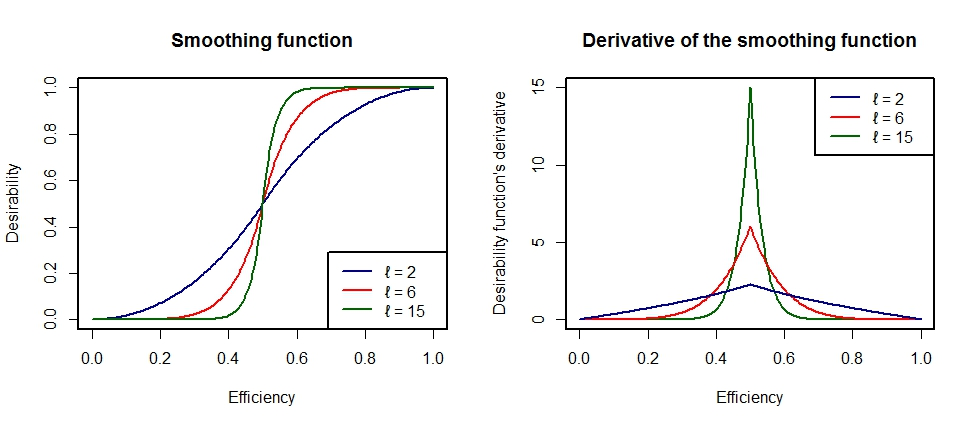
\includegraphics[width=\textwidth]{DesFunPlot.jpg}
\caption{Desirability function parameterisation and its derivative}
\label{Fig::des_fun}
\end{center}
\end{figure}
It can be seen that the function increases slowly at first and then, after a certain value depending on the parameter $l$ it makes a very sharp jump (larger values of $l$ correspond to faster jumps) and slowly reaches its maximum. This particular parameterisation makes the desirability function most sensitive to the changes of the efficiencies around $0.5$ which should result in considerable prevalence of the designs which are more than $50\%$ efficient. The value of $l$ was chosen to be equal to $6$ as a compromise between the slow and fast desirability increase rates in the middle region.

\subsection{Optimal designs}
The optimum design search was implemented for the first example described earlier: a three-factor experiment with each factor comprising three levels; with $40$ runs and $p=21$ parameters in the full quadratic polynomial model. As before, the interest is in all parameters except for the intercept; and the point exchange algorithm was used to find the designs maximising the following criterion function:
\begin{multline*}
\left[f(\mbox{Eff}_D(\bm{X}))\right]^{\kappa_D}\left[f(\mbox{Eff}_{DP}(\bm{X}))\right]^{\kappa_{DP}}\left[f(\mbox{Eff}_{DF}(\bm{X}))\right]^{\kappa_{DF}}\left[f(\mbox{Eff}_{LoF}(\bm{X}))\right],^{\kappa_{LoF}}
\end{multline*}
where the non-negative weights are to follow the same restriction as before: 
\begin{equation*}
\kappa_{D}+\kappa_{DP}+\kappa_{DF}+\kappa_{LoF}=1.
\end{equation*} 

Since here we utilise the function of the efficiencies at each step of the search, before using any composite criterion it is necessary to obtain optimality values of the elementary criteria involved: $D$, $DP$, $L$, $LP$, $DF$ and $LoF$ (the latter two are quite apparent, though), as we cannot just calculate the criteria functions directly when searching for the design. In this particular case we take the same $f(x)$ for every component, however, of course, different forms of the desirability function can be used as long as they are constructed appropriately and satisfy the restrictions (i.e. defined for all $x\in[0,1]$ and $f:[0,1]\rightarrow[0,1]$).    
 
The results for the determinant and trace-based criteria are summarised in Tables \ref{Table_DesFunD} and \ref{Table_DesFunL} respectively, where, as before, the efficiencies of the designs in terms of various primary criteria are given together with the allocation of residual degrees of freedom between the pure error and lack-of-fit components. It can be noticed that this parameterisation is rather sensitive and allows finding the best or almost the best designs; the $D$-efficiency for the `$D$-optimal' design \#$1$ is equal to $99.79\%$ ($99.61\%$ for the `$L$-optimal').

\begin{table}[h]
\centering
\caption{Example 1. Properties of optimal designs in terms of determinant-based compound criteria constructed with desirability functions}
\label{Table_DesFunD}
\scalebox{0.8}{
%\resizebox{\textwidth}{!}} \\
 & \textbf{D} & \textbf{DP} & \textbf{DF} & \textbf{LoF} & \textbf{PE} & \textbf{LoF} & \textbf{D} & \textbf{DP} & \textbf{L} & \textbf{LP} & \textbf{LoF} & \textbf{DF} \\
1 & 1 & 0 & 0 & 0 & 0 & 19 & 99.79 & 0.00 & 99.42 & 0.00 & 0.00 & 100.00\\
2 & 0 & 1 & 0 & 0 & 18 & 1 & 92.81 & 99.79 & 79.26 & 92.94 & 66.00 & 55.00\\
3 & 0.5 & 0.5 & 0 & 0 & 15 & 4 & 96.15 & 97.31 & 84.34 & 96.09 & 95.35 & 62.50\\
4 & 0.5 & 0 & 0.5 & 0 & 0 & 19 & 99.95 & 0.00 & 100.00 & 0.00 & 0.00 & 100.00\\
5 & 0.5 & 0 & 0 & 0.5 & 11 & 8 & 97.87 & 87.11 & 91.53 & 97.79 & 98.83 & 72.50\\
6 & 0 & 0.5 & 0.5 & 0 & 9 & 10 & 98.36 & 78.90 & 94.32 & 95.40 & 92.86 & 77.50\\
7 & 0 & 0.5 & 0 & 0.5 & 14 & 5 & 96.93 & 95.61 & 87.27 & 98.19 & 98.48 & 65.00\\
8 & 0 & 0 & 0.5 & 0.5 & 8 & 11 & 45.20 & 33.80 & 17.06 & 16.60 & 87.94 & 80.00\\
9 & 1/3 & 1/3 & 1/3 & 0 & 9 & 10 & 98.42 & 78.95 & 93.63 & 94.70 & 92.86 & 77.50\\
10 & 1/3 & 1/3 & 0 & 1/3 & 9 & 10 & 98.42 & 78.95 & 93.63 & 94.70 & 92.86 & 77.50\\
11 & 0 & 1/3 & 1/3 & 1/3 & 9 & 10 & 98.30 & 78.95 & 94.19 & 95.26 & 92.86 & 77.50\\
12 & 0.25 & 0.25 & 0.25 & 0.25 & 9 & 10 & 98.36 & 78.90 & 94.32 & 95.40 & 92.86 & 77.50\\
\end{tabular}
}
\end{table}

In general, comparing with the designs in the previous section, the distribution of the residual degrees of freedom was affected by using the desirability functions: now the numbers of pure error degrees of freedom is generally smaller, so often more of the available degrees of freedom are allocated to the lack-of-fit. Even the criterion \#$8$, whose value depends only on the degrees of freedom, in this case does not provide the best result: $8$ instead of the optimal $10$ pure error degrees of freedom. 

The current parameterisation provides quite large impact for the efficiency values around $50-80\%$, and one of the consequences is that the search may stop while in reality finding a considerably worse design. For example, design \#$10$ (the same as \#$9$) in Table \ref{Table_DesFunD} is $78.95\%$ $DP$-efficient, as the efficiency of the real optimal design according to this composite criterion, with $1/3$ allocated to the $DP$-component, is $95.61\%$ (as in Table \ref{Table_extraFD}). The fact is that the desirability function (\ref{eq::des_fun_exp}) $f(0.7895)=0.9972$, i.e. the transformed efficiency of $99.72\%$ is actually larger than the `true' one. In the meantime, the $D$-efficiency has increased by approximately $1.5\%$ (the corresponding weight is $1/3$ as well); and the current design contains fewer replicates, the number of pure error degrees of freedom is equal to $9$ in comparison to $14$ obtained previously (Table \ref{Table_extraFD}).

\begin{table}[h]
\centering
\caption{Example 1. Properties of optimal designs in terms of trace-based compound criteria constructed with desirability functions}
\label{Table_DesFunL}
\scalebox{0.8}{
%\resizebox{\textwidth}{!}} \\
 & \textbf{L} & \textbf{LP} & \textbf{DF} & \textbf{LoF} & \textbf{PE} & \textbf{LoF} & \textbf{D} & \textbf{DP} & \textbf{L} & \textbf{LP} & \textbf{LoF} & \textbf{DF} \\
1 & 1 & 0 & 0 & 0 & 0 & 19 & 99.03 & 0.00 & 99.61 & 0.00 & 0.00 & 100.00\\
2 & 0 & 1 & 0 & 0 & 13 & 6 & 96.49 & 92.44 & 90.04 & 99.85 & 99.93 & 67.50\\
3 & 0.5 & 0.5 & 0 & 0 & 9 & 10 & 96.91 & 77.74 & 94.53 & 95.61 & 92.86 & 77.50\\
4 & 0.5 & 0 & 0.5 & 0 & 0 & 19 & 99.71 & 0.00 & 99.60 & 0.00 & 0.00 & 100.00 \\
5 & 0.5 & 0 & 0 & 0.5 & 10 & 9 & 96.91 & 82.29 & 93.99 & 97.98 & 96.46 & 75.00 \\
6 & 0 & 0.5 & 0.5 & 0 & 6 & 13 & 98.17 & 59.69 & 96.83 & 83.70 & 73.27 & 85.00\\
7 & 0 & 0.5 & 0 & 0.5 & 13 & 6 & 95.49 & 91.47 & 89.99 & 99.79 & 99.93 & 67.50\\
8 & 0 & 0 & 0.5 & 0.5 & 8 & 11 & 45.20 & 33.80 & 17.06 & 16.60 & 87.94 & 80.00 \\
9 & 1/3 & 1/3 & 1/3 & 0 & 6 & 13 & 98.56 & 59.92 & 96.91 & 83.77 & 73.27 & 85.00\\
10 & 1/3 & 1/3 & 0 & 1/3 & 10 & 9 & 96.91 & 82.29 & 93.99 & 97.98 & 96.46 & 75.00 \\
11 & 0 & 1/3 & 1/3 & 1/3 & 8 & 11 & 96.75 & 72.34 & 95.35 & 92.80 & 87.94 & 80.00 \\
12 & 0.25 & 0.25 & 0.25 & 0.25 & 8 & 11 & 97.99 & 73.27 & 95.41 & 92.87 & 87.94 & 80.00 
\end{tabular}
}
\end{table}
 

However, as most of the efficiencies lie either below $10\%$ or far above $75\%$, the effect of making the criteria sensitive to the changes within the middle of the interval cannot be frequently observed here; in the case of trace-based criteria, efficiency losses do not exceed $5\%-7\%$.

The results for the second example of a four five-level factorial experiment with $60$ runs, and $p=15$ model parameters (as introduced in the previous section), are given in Appendix \ref{appendix::DesFun}. Efficiency drops can be observed in the case of determinant-based criteria as well (although less drastic than in the first example), designs also tend to have fewer replicates. In addition, quite a few designs were found to be optimal with respect to different criteria; this could be explained by the fact that in the process of point exchanges the algorithm might come across some designs sooner/more often and stop the search due to the nature of the desirability function parameterisation that magnifies the impact of efficiency values from a certain sub-interval.


\section{Conclusions}
In this chapter we explored some extensions and amendments to the previously developed compound criteria, that is adding an extra F-quantile in order to guarantee some degrees of freedom for the purposes of statistical inference and considering transformed efficiencies as the criteria components that allows tailoring the form of each component's impact on the overall design performance.

Adding another F-quantile does serve the purpose it was implemented for (especially in the case of trace-based criteria). However, the issue of interpretation and the sensibility of introducing a whole new component just for this particular aim that seems to be `correlated' with the effects of other components, are quite questionable. 

It was desired to alter the form of an efficiency's contribution in the compound criteria values by using desirability functions of the efficiencies as the individual components of the criteria. And although the desirability functions that have been considered can certainly be useful for specific applications, they do not provide the best flexibility for these particular criteria. As the efficiency of the majority of optimal designs lie in the upper range of the $[0,1]$ interval, it makes sense to `shift' this jump (linear or as in (\ref{eq::des_fun_exp})) towards the larger values of the argument. Such asymmetrical parameterisations might be a better option as a generally suitable alternative to the common approach; it has not been investigated yet, but would be worth examining and adapting for some particular practical requirements that might be in place.   